\documentclass[a4paper,11pt]{article}

\usepackage[english,greek]{babel}

\newcommand{\gt}{\greektext}
\newcommand{\lt}{\latintext}

\usepackage{amsmath}
\usepackage[pdftex]{graphicx}
\usepackage{verbatim}  
\usepackage{graphicx}
\usepackage{hyperref}

\title{2η Υποχρεωτική Εργασία \\ Στο Μάθημα της Αριθμητικής Ανάλυσης}
\author{Όνοματεπώνυμο: Γεώργιος Κεσογλίδης  \\  ΑΕΜ: 3911}
\date{\today}                                     

\begin{document}

\maketitle
H υλοποίηση όλων των ασκήσεων πραγματοποιήθηκε στην \lt python. \gt

\section{Άσκηση 5}

Το ημίτονο έχει περιόδο ίση με 2π. Άρα χρείαζεται μόνο να προσεγγίσουμε τις τιμές του ημιτόνου στο διάστημα [-π ,π] για να υπολογίσουμε την ολική συνάρτηση. \\
Χρησιμοποιούμε 10 ομοιομορφά κατανεμημένα σημεία στο [-π,π]

\subsection{Πολυωνυμική προσέγγιση - \lt Lagrange}
Με τους παρακάτω τύπους υπολογίζουμε το πολυωνυμο παρεμβολής του \lt Lagrange \gt
\begin{equation*}
p_n(x) = \sum_{i=0}^{n}y_iL_i(x)
\end{equation*}
\begin{center}
όπου
\end{center}
\begin{equation*}
L_i(x) = \frac{(x-x_0)...(x-x_{i-1})(x-x_{i+1})...(x-x_n)}{(x_i-x_0)...(x_i-x_{i-1})(x_i-x_{i+1})...(x_i-x_n)}
\end{equation*}
Το γράφημα του σφάλματος του πολυωνύμου \lt Lagrange \gt είναι το εξής:. \\ \\
\hspace*{-2 cm}
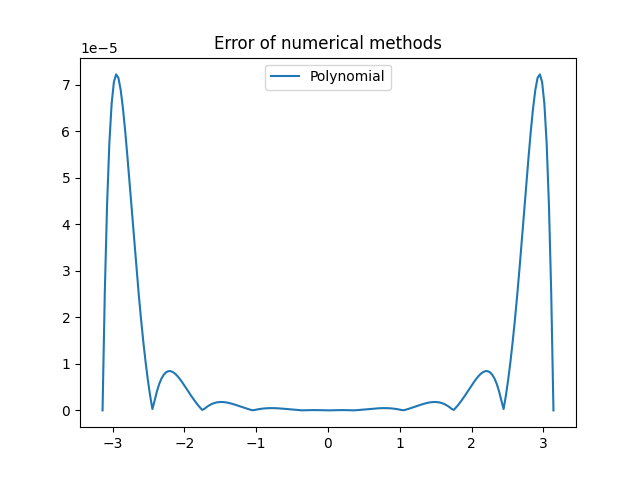
\includegraphics[scale=1]{poly.png}
Από το γράφημα βλέπουμε ότι το μέγιστο σφάλμα είναι μικρότερο του 0.0001. Άρα η ακριβεία που έχουμε είναι 4 δεκαδικά ψηφία. Επίσης, παρατηρούμε ότι το σφάλμα είναι πολύ μεγαλύτερο στις άκρες του διαστήματος. Αυτό οφείλεται στο φαινόμενο του Ρούνγκε \lt - Runge. \gt

\subsection{Κυβικα - \lt Cubic Splines}
Η συγκεκριμένη μέθοδος βρίσκει ν -1 κυβικά πολυώνυμα για ν δεδομένα. Το κυβικό πολυώνυμο έχει την εξής μορφή:
\begin{equation*}
y = ax^3 + bx^2 + cx + d
\end{equation*}
Άρα έχουμε 4(ν -1) αγνώστους που πρέπει να υπολογίσουμε. Για να είναι εφικτή η εύρεση αυτών ορίζουμε τους παρακάτω περιορισμούς και λύνουμε το γραμμικό σύστημα που προκύπτει.

\begin{equation*}
S_i(x_i)=y_i, 
\quad \quad \quad \quad \quad \quad  \quad
i=1,…,n-1
\end{equation*}
\begin{equation*}
S_i(x_{i+1})=y_{i+1},
\quad \quad  \quad \quad \quad i=1,…,n-1
\end{equation*}
\begin{equation*}
S^{'}_i(x_{i+1})=S^{'}_{i+1}(x_{i+1}), 
\quad \quad i=1,…,n-2
\end{equation*}
\begin{equation*}
S^{''}_i(x_{i+1})=S^{''}_{i+1}(x_{i+1}),
\quad \quad i=1,…,n-2
\end{equation*}
\begin{equation*}
S^{''}_1(x_1)=0 \quad \quad \quad \quad \quad \quad \quad \quad \quad \quad \quad \quad \quad \quad
\end{equation*}
\begin{equation*}
S^{''}_{n-1}(x_n)=0 \quad \quad \quad \quad \quad \quad \quad \quad \quad \quad \quad \quad \quad 
\end{equation*}

Χρησιμοποιούμε κυβικά \lt splines \gt διότι προσφέρουν αρκετή λεπτομέρεια ενώ ταυτόχρονα αποφεύγουν το φαινόμενο του Ρούνγκε \lt - Runge. \gt \\
Το γράφημα του σφάλματος της \lt splines \gt είναι το εξής:. \\

\hspace*{-2.7 cm}
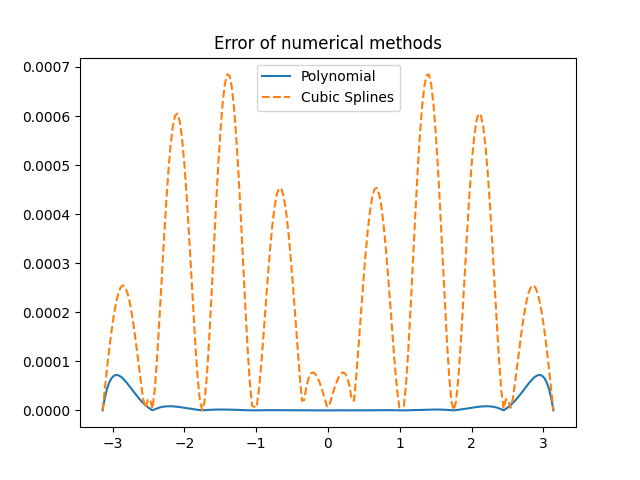
\includegraphics[scale=1]{splines.png}
Από το γράφημα βλέπουμε ότι το μέγιστο σφάλμα είναι μικρότερο του 0.001. Άρα η ακρίβεια που έχουμε είναι 2 δεκαδικά ψηφία.

\newpage
\subsection{Μέθοδος ελαχίστων τετραγώνων}
Στην μέθοδο ελαχίστων τετραγώνων χρησιμοποιούμε κάποια απλή συνάρτηση για να προσεγγίσουμε μία πιο περίπλοκη. Συγκεκριμένα, θα χρησιμοποιήσουμε κάποιο πολυώνυμο με βαθμό μικρότερο από το πλήθος των δεδομένων που μας δίνονται για να προσεγγίσουμε την συνάρτηση του ημιτόνου. Για να υπολογίσουμε τους συντελέστες του πολυωνύμου θα  λύσουμε ως προς \lt x \gt το εξής σύστημα:
\begin{equation*}
A^TAx = A^Tb
\end{equation*}
όπου 
\begin{itemize}
\item Α ο πίνακας που κάθε γραμμή αντιστοιχεί σε μία από τις δεδομένες τιμές και κάθε στήλη αντιστοιχεί στην δεδομένη τιμή υψωμένη εις την αντίστοιχη στήλη από 0 εώς τον βαθμό του πολυωνύμου
\item \lt x \gt οι συντελεστές του πολυωνύμου
\item \lt b \gt τα αποτελέσματα της συνάρτησης του ημιτόνου στις δεδομένες τιμές
\end{itemize}
Ύστερα από δοκιμές βρήκαμε ότι η μέθοδος ελαχίστων τετραγώνων για την συνάρτηση του ημιτόνου παράγει χρήσιμες προσεγγίσεις για πολυώνυμα μεγαλύτερα ή ισά του πέμπτου βαθμού.
Διότι για μικρότερους βαθμούς δεν έχουμε ακρίβεια για κανένα δεκαδικό ψηφίο.
Το σφάλμα της μεθόδου ελαχίστων τετραγώνων φαίνεται στο γράφημα. \\
\hspace*{-2 cm}
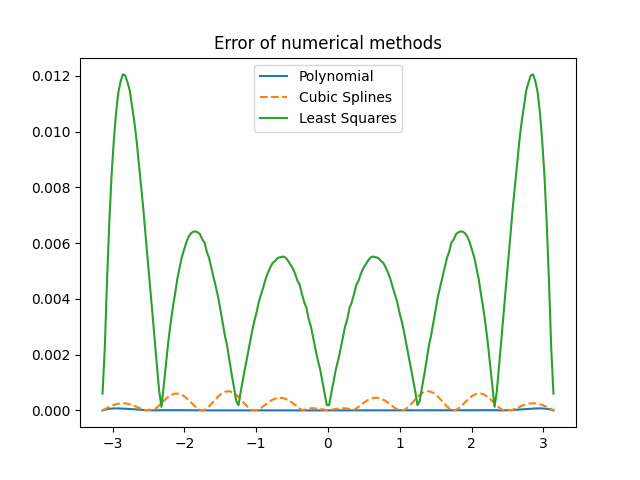
\includegraphics[scale=1]{ls.png}
Από το γράφημα βλέπουμε ότι το μέγιστο σφάλμα είναι περίπου 0.012.  Άρα η ακριβεία που έχουμε είναι 1 δεκαδικό ψηφίο. Θα μπορούσαμε να πετύχουμε μεγαλύτερη ακρίβεια για μεγαλύτερου βαθμού πολυώνυμα που ο βαθμός δεν ξεπερνά το πλήθος των δεδομένων

\newpage
\section{Άσκηση 6}
Υπολογίζουμε αλγεβρικά το ολοκλήρωμα της συνάρτησης του ημιτόνου στο διάστημα [0, π/2].
\begin{equation*}
\int^{\frac{\pi}{2}}_{0}sin(x)dx 
= [-cos(x)]^{\frac{\pi}{2}}_0
= -cos(\frac{\pi}{2}) + cos(0) = 1
\end{equation*}
Τώρα θα υπολογίσουμε την τιμή προσσεγιστικά
\subsection{Μέθοδος του τραπεζίου}
Για Ν+1 σημεία στο διάστημα \lt [a,b] \gt προκύπτουν Ν τραπέζια. \\
Χρησιμοπιούμε τον τύπο της μεθόδου του τραπεζίου
\begin{equation*}
\frac{b-a}{2N}(f(x_0)+f(x_N)+2\sum^{N-1}_{k=1}f(x_k)
\end{equation*}
Το σφάλμα προσέγγισης θεωρητικά είναι:
\begin{equation*}
M = max\{|f^{''}(x)|\} = max\{-sin(x)\} = 1
\end{equation*}

\begin{equation*}
|e| \leq \frac{(b-a)^3}{12N^2}M 
= \frac{(\frac{\pi}{2})^3}{12*10^2}1 
= \frac{\pi^3}{9600} = 0.00322982048 < 10^{-2}
\end{equation*}
Άρα έχουμε 2 δεκαδικά ψηφία ακρίβειας.
Ενώ το σφάλμα προσέγγισης αριθμητικά είναι: 
\begin{equation*}
|1 - 0.9979429863543572| = 0.00205701364 < |e|
\end{equation*}
Είναι λογικό ότι το αριθμητικό σφάλμα προσέγγισης είναι μικρότερο από το θεωρητικό διότι το θεωρητικό σφάλμα είναι το μέγιστο εφικτό.

\newpage
\subsection{Μέθοδος \lt Simpson}
Χρησιμοποιούμε τον τύπο της μεθόδου \lt Simpson. \gt
\begin{equation*}
\frac{b-a}{3N}(f(x_0)+f(x_N)+2\sum^{\frac{N}{2}-1}_{i=1}f(x_{2i}) + 4\sum^{\frac{N}{2}}_{i=1}f(x_{2i-1})
\end{equation*}
όπου
\begin{itemize}
\item \lt b – a \gt = µήκος διαστήµατος ολοκλήρωσης 
\item Ν = πλήθος υποδιαστηµάτων = πλήθος σηµείων – 1
\end{itemize}
Το σφάλμα προσέγγισης θεωρητικά είναι:

\begin{equation*}
M = max\{|f^{4}(x)|\} = max\{sin(x)\} = 1
\end{equation*}

\begin{equation*}
|e| \leq \frac{(b-a)^5}{180N^4}M 
= \frac{(\frac{\pi}{2})^5}{180*10^4}1 
= \frac{\pi^5}{5760*10^4} 
= 0.00000531284 < 10^{-5}
\end{equation*}
Άρα έχουμε 5 δεκαδικά ψηφία ακρίβειας.
Ενώ το σφάλμα προσέγγισης αριθμητικά είναι: 
\begin{equation*}
|1 - 1.0000033922209004| = 
0.00000339222 < 0.34 *10^{-5} < |e|
\end{equation*}
Είναι λογικό ότι το αριθμητικό σφάλμα προσέγγισης είναι μικρότερο από το θεωρητικό διότι το θεωρητικό σφάλμα είναι το μέγιστο εφικτό.

\newpage
\section{Άσκηση 7}
Επιλέξαμε τις μετοχές \\
\begin{enumerate}
\item \lt HELLENIQ ENERGY \gt ΑΝΩΝ. ΕΤΑΙΡ. ΣΥΜΜΕΤΟΧΩΝ 
\item \lt INTRAKAT \gt ΑΝΩΝΥΜΟΣ ΕΤΑΙΡΕΙΑ (ΙΝΚΑΤ)\end{enumerate}
και πήραμε τις τίμες κλεισίματος από το \lt
\url{https://www.capital.gr/finance/historycloses} \gt
για τις ημερομηνίες 29/09/2022 (29 Σεπτεμβρίου 2022) εώς 12/10/2022 (12 Οκτωβρίου 2022). Ο σκοπός αυτών των επιλογών ήταν να μελετήσουμε μία μετοχή (ΕΛΠΕ) της οποίας η τιμή αυξάνεται ομαλά, δηλαδή κυρίως αυξάνεται, και μίας άλλης (ΙΝΚΑΤ) της οποίας η τιμή μειώνεται μη ομαλά δηλαδή αυξομειώνεται αλλά στο τέλος παρατηρείται μείωση. \\
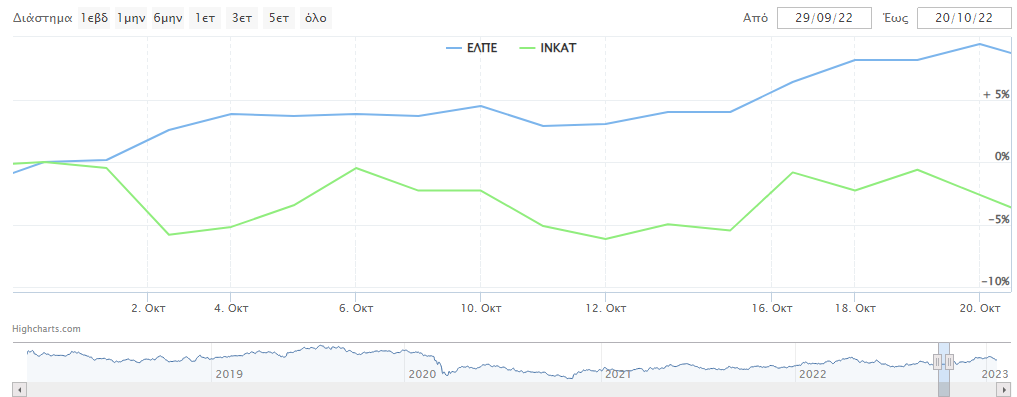
\includegraphics[scale=0.48]{stocks.png}
Με αυτές τις τιμές ως δεδομένα θα εφαρμόσουμε την μέθοδο ελαχίστων τετραγώνων, με πολυώνυμο 2ου, 3ου και 4ου βαθμού, για να προσεγγίσουμε την συνάρτηση τιμής κλεισίματος. Στην συνέχεια θα βρούμε τις τιμές των συναρτήσεων για τις ημέρες: \begin{itemize}
\item 13/10/2022 (13 Οκτωβρίου 2022) 
\item  20/10/2022 (20 Οκτωβρίου 2022)
\end{itemize}

\subsection{ΕΛΠΕ}
\subsubsection{Πρόβλεψη επόμενης συνεδρίασης 13/10/2022 \\ (13 Οκτωβρίου 2022)}
\lt 
For Elpe \\
13/10/2022 actual price: 6.5 \\
2nd /3rd /4th degrees predictions\\
6.3578 /6.3843 /6.4658 \gt \\
Το τετάρτου βαθμού πολυώνυμο βρίσκει την πιο κοντινή τιμή
\subsubsection{Πρόβλεψη πέντε συνεδριάσεων μετά 20/10/2022 \\ (20 Οκτωβρίου 2022)}
\lt 20/10/2020 actual price: 6.84 \\
2nd /3rd /4th degrees predictions\\
5.7936 /6.1036 /8.4648 \\
\gt
Το τρίτου βαθμού πολυώνυμο βρίσκει την πιο κοντινή τιμή

\subsection{ΙΝΚΑΤ}

\subsubsection{Πρόβλεψη επόμενης συνεδρίασης 13/10/2022 \\ (13 Οκτωβρίου 2022)}
\lt For Inkat \\
13/10/2022 actual price 1.372 \\
2nd /3rd /4th degrees predictions\\
1.3684 /1.2616 /1.3026 \\
\gt
Το δευτέρου βαθμού πολυώνυμο βρίσκει την πιο κοντινή τιμή

\subsubsection{Πρόβλεψη πέντε συνεδριάσεων μετά 20/10/2022 \\ (20 Οκτωβρίου 2022)}
\lt 
20/10/2020 actual price 1.406 \\
2nd /3rd /4th degrees predictions \\
1.3345 /0.086 /1.2724 \gt \\
Το δευτέρου βαθμού πολυώνυμο βρίσκει την πιο κοντινή τιμή

\subsection{Σύνοψη}
Παρόλο που κάποιες προβλέψεις τυχαίνει να βρίσκονται κοντά στην πραγματική τιμή τα δεδομένα μας είναι παρα πολύ λίγα και οι παράγοντες που επηρεάζουν την τιμή κλεισίματος μιας μετοχής πάρα πολλοί για να μπορούμε να κατασκευάσουμε μία καλή προσέγγιση.
\end{document}